% !arara: pdflatex: { shell: on, interaction: nonstopmode }
% !arara: biber
% arara: pdflatex: { interaction: nonstopmode }
% arara: pdflatex: { interaction: nonstopmode }
% --------------------------------------------------------------------------
% the TRANSLATIONS package
% 
%   internationalization of LaTeX packages
% 
% --------------------------------------------------------------------------
% Clemens Niederberger
% Web:    https://github.com/cgnieder/translations
% E-Mail: clemens@cnltx.de
% --------------------------------------------------------------------------
% Copyright 2012--2022 Clemens Niederberger
% 
% This work may be distributed and/or modified under the
% conditions of the LaTeX Project Public License, either version 1.3c
% of this license or (at your option) any later version.
% The latest version of this license is in
%   http://www.latex-project.org/lppl.txt
% and version 1.3c or later is part of all distributions of LaTeX
% version 2008/05/04 or later.
% 
% The Current Maintainer of this work is Clemens Niederberger.
% --------------------------------------------------------------------------
\documentclass{translations-manual}

\begin{document}

\part{Preface}

\section{Motivation}
This package provides means for package authors to have an easy interface for
internationalization of their packages.  The functionality of this package is
in many parts also covered by the package
\pkg{translator}~\cite{pkg:translator} (which used to be part of the
\pkg*{beamer} bundle).  Internationalization is also possible with
\pkg{babel}~\cite{pkg:babel} and it's \cs*{addto}\cs*{captions\meta{language}}
mechanism or \KOMAScript's \cs*{providecaptionname} and similar commands.
However, I believe that \translations\ is more flexible than all of these.
Unlike \pkg{translator} it detects the used (\pkg{babel} or
\pkg{polyglossia}~\cite{pkg:polyglossia}) language itself and provides
expandable retrieving of the translated key.  \translations\ also provides
support for language dialects which means package authors can for example
distinguish between British, Australian, Canadian and US~English.

The first draft of the package was written since I missed an expandable
version of \pkg{translator}'s \cs*{translate} command. Initially the package
was part of my \pkg{exsheets} bundle~\cite{pkg:exsheets}. However, once I had
the package available I began using it in various of my other packages and it
got extended to the needs I faced there.  In the end it made sense to
distribute it as package of its own.

\section{License}\label{sec:license}
\license

\part{Usage}
\section{Background}
The \translations\ package enables the author of a package or a class (or a
document) to declare translations of key words in different languages and
fetch these translations in the document depending on the active language as
set by \pkg{babel} or \pkg{polyglossia}.  Since \translations\ checks which
language is active it is generally not necessary (although possible) to
specify the language for which a translation should be fetched manually.

\translations\ knows of two types of languages: main languages (see
\cref{tab:languages} on \cpageref{tab:languages}) and language dialects (see
\cref{tab:dialects} on \cpageref{tab:dialects}).

\translations\ also knows language aliases (see \cref{tab:aliases} on
\cpageref{tab:aliases}).  For the commands declaring or fetching a translation
languages\slash dialects and their aliases are equivalent.

\Cref{fig:scheme} demonstrates what happens if \translations\ is asked to
fetch a translation for a given key.

\begin{figure}[htbp]
  \newcommand*\yes{\centering\textcolor{green}{\CheckmarkBold}\par}
  \newcommand*\no{\centering\textcolor{red}{\XSolidBrush}\par}
  \centering
  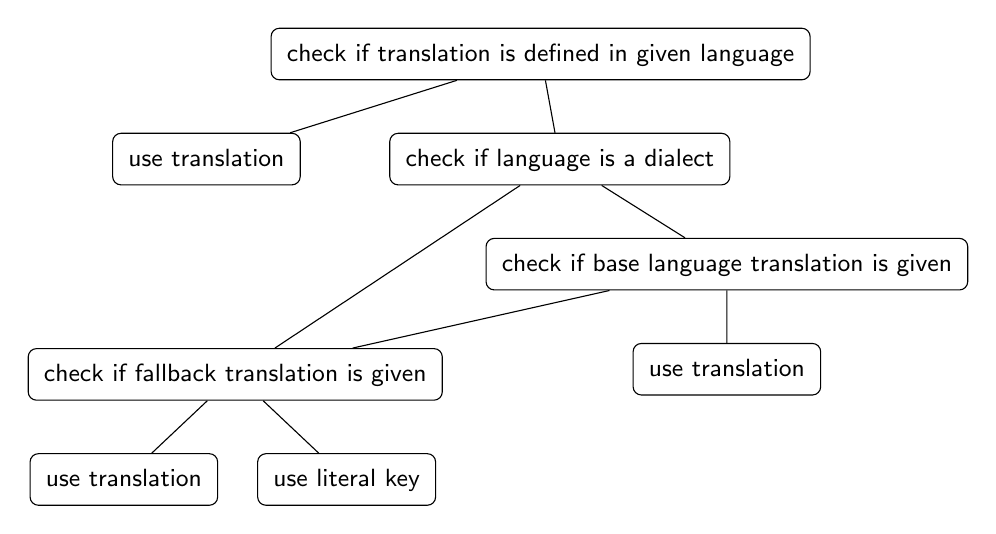
\begin{tikzpicture}
    [
      level/.style={sibling distance=.7\linewidth/#1,level distance=10mm},
      every node/.style={
        draw,
        rounded corners=3pt,
        align=left,
        anchor=north,
        font=\small\sffamily,
        inner sep = 2mm ,
        text depth = 1pt
      }
    ]
    \node {check if translation is defined in given language}
      child { node {\yes use translation} }
      child {
        node[xshift=-4cm] {\no check if language is a dialect}
        child[level distance=24mm] {
          node[xshift=-2cm] (fallback) {\no check if fallback translation is given}
          child { node {\yes use translation} }
          child { node {\no use literal key} }
        }
        child {
          node (base) {\yes check if base language translation is given}
          child { node {\yes use translation} }
        }
      } ;
    \draw (base) -- (fallback) ;
  \end{tikzpicture}
  \caption{Schematic representation of \translations' translating mechansim.}
  \label{fig:scheme}
\end{figure}

What happens if you declare a translation?
\begin{enumerate}
  \item You declare a translation for a base language: this is the normal case
    where an internal macro is defined which can be fetched by the
    \cs{GetTranslation} command (see \cref{ssec:commands}).  This translation
    is also used for dialects of the base language if the dialect translation
    has not been defined.
  \item You declare a translation for a dialect: this is more or less the
    same, except the translation is not used for any other cases.
  \item You declare a translation for a language alias: this is the very same
    as the other cases, depending on wether its the alias of a base language
    or a dialect.
\end{enumerate}
This means that if the document language is a base language (\emph{English}
for example) and there is a translation for a dialect (\emph{British} for
example) but not for the base language then no translation is found.  If the
situation is the other way around (the document language is \emph{British} and
a translation for \emph{English} exists but not for \emph{British}) then the
translation for the base language is found and used.

\begin{bewareofthedog}
  Beware that if the current language is a language using a non-latin font, a
  translation is missing for said language, and the fallback translation needs
  a Latin script font then \emph{nothing} might be printed.
\end{bewareofthedog}

\section{Available Commands}\label{ssec:commands}
Below the commands provided by \translations\ are explained.  The symbol
\textcolor{expandable}{\expandablesign} means that the command is expandable.
Commands without the marker aren't expandable.

\begin{commands}
  \command{DeclareLanguage}[\marg{language}]
    Declare a language that can be used by \translations.  If the language
    already exists it will be silently redefined.  This command can only be
    used in the preamble.  It should never be necessary to use this command as
    \translations\ already declares loads of languages (\cref{sec:languages}).
    Should you miss one please send me an email and I'll add it to
    \translations.
  \command{DeclareLanguageAlias}[\marg{language2}\marg{language1}]
    Declares \meta{language2} to be an alias of \meta{language1}.  If
    \meta{language1} doesn't exist yet a warning will be raised and it will be
    defined.  This command can only be used in the preamble.  It should never
    be necessary to use this command as \translations\ already declares loads
    of languages (\cref{sec:languages}).  Should you miss one please send me
    an email and I'll add it to \translations.
  \command{DeclareLanguageDialect}[\marg{dialect}\marg{language}]
    Declares \meta{dialect} to be a dialect of language \meta{language}.  If a
    translation for \meta{dialect} is provided it is used by the translation
    macros.  If there is none the corresponding translation for \meta{language}
    is used instead.  It should never be necessary to use this command as
    \translations\ already declares loads of languages (\cref{sec:languages}).
    Should you miss one please send me an email and I'll add it to
    \translations.
  \command{NewTranslation}[\marg{language}\marg{key}\marg{translation}]
    Defines a translation of key \meta{key} for the language \meta{language}.
    An error will be raised if a translation of \meta{key} in language
    \marg{language} already exists. This command can only be used in the
    preamble.
  \command{NewTranslationFallback}[\marg{key}\marg{translation}]
    \sinceversion{1.4}Defines a fallback translation of key \meta{key} for the
    language \meta{language}. An error will be raised if a fallback translation of
    \meta{key} already exists. This command can only be used in the preamble.
  \command{RenewTranslation}[\marg{language}\marg{key}\marg{translation}]
    Redefines a translation of key \meta{key} for the language \meta{language}.
    An error will be raised if no translation of \meta{key} in language
    \meta{language} exists.  This command can only be used in the preamble.
  \command{RenewTranslationFallback}[\marg{key}\marg{translation}]
    \sinceversion{1.4}Renews a fallback translation.  This command can only be
    used in the preamble.
  \command{ProvideTranslation}[\marg{language}\marg{key}\marg{translation}]
    \sinceversion{1.2}Provides a translation of key \meta{key} for the
    language \meta{language}. If a translation of \meta{key} in language
    \meta{language} already exists it won't be overwritten and no error will be
    raised.  This command can only be used in the preamble.
  \command{ProvideTranslationFallback}[\marg{key}\marg{translation}]
    \sinceversion{1.4}Provides a fallback translation.  This command can only
    be used in the preamble.
  \command{DeclareTranslation}[\marg{language}\marg{key}\marg{translation}]
    Defines a translation of key \meta{key} for the language \meta{language}.
    No error will be raised if a translation of \meta{key} already exists.
    This command can only be used in the preamble.
  \command{DeclareTranslationFallback}[\marg{key}\marg{fallback}]
    Declares a fallback translation.  This command can only be used in the
    preamble.
  \command{definetranslation}[\marg{language}\marg{key}\marg{translation}]
    \sinceversion{1.4}A version of \cs{NewTranslation} that \emph{can} be used
    after begin document.
  \command{definetranslationfallback}[\marg{key}\marg{translation}]
    \sinceversion{1.4}A version of \cs{NewTranslationFallback} that \emph{can}
    be used after begin document.
  \command{redefinetranslation}[\marg{language}\marg{key}\marg{translation}]
    \sinceversion{1.4}A version of \cs{RenewTranslation} that \emph{can} be
    used after begin document.
  \command{redefinetranslationfallback}[\marg{key}\marg{translation}]
    \sinceversion{1.4}A version of \cs{RenewTranslationFallback} that
    \emph{can} be used after begin document.
  \command{addtranslation}[\marg{language}\marg{key}\marg{translation}]
    \sinceversion{1.4}A version of \cs{ProvideTranslation} that \emph{can} be
    used after begin document.
  \command{addtranslationfallback}[\marg{key}\marg{translation}]
    \sinceversion{1.4}A version of \cs{ProvideTranslationFallback} that
    \emph{can} be used after begin document.
  \command{declaretranslation}[\marg{language}\marg{key}\marg{translation}]
    \sinceversion{1.4}A version of \cs{DeclareTranslation} that \emph{can} be
    used after begin document.
  \command{declaretranslationfallback}[\marg{key}\marg{translation}]
    \sinceversion{1.4}A version of \cs{DeclareTranslationFallback} that
    \emph{can} be used after begin document.
  \expandable\command{IfTranslation}[\marg{language}\marg{key}\marg{true}\marg{false}]
    Checks\sinceversion{1.2d} if a translation for \meta{key} in language
    \meta{language} is defined or not and either leaves \meta{true} or
    \meta{false} in the input stream.
  \expandable\command{GetTranslationFor}[\marg{language}\marg{key}]
    Fetches and prints the translation of \meta{key} for the language
    \meta{language}.  This command is expandable.
  \expandable\command{GetTranslation}[\marg{key}]
    Fetches and prints the translation of \meta{key} for the currently active
    language (as for example set by \pkg{babel}).  This command is expandable.
  \command{GetTranslationForWarn}[\marg{language}\marg{key}]
    \sinceversion{1.0}Fetches and prints the translation of \meta{key} for
    the language \meta{language}.  Issues a warning if no translation is
    available at the cost of expandability.
  \command{GetTranslationWarn}[\marg{key}]
    \sinceversion{1.0}Fetches and prints the translation of \meta{key} for
    the currently active language (as for example set by \pkg{babel}).
    Issues a warning if no translation is available at the cost of
    expandability.
  \command{SaveTranslation}[\marg{cmd}\marg{key}]
    Fetches and saves the translation of \meta{key} for the currently active
    language (as for example set by \pkg{babel}) in the macro \meta{cmd}.
  \command{LoadDictionary}[\marg{name}]
    Loads a file named \code{\meta{name}-\meta{language}.trsl} where \meta{language}
    corresponds to the lowercase name of the current language as defined with
    \cs{DeclareLanguage}.  This file should contain the translations for the
    specified language.
  \command{LoadDictionaryFor}[\marg{language}\marg{name}]
    Loads a file named \code{\meta{name}-\meta{language}.trsl}.
  \command{NewDictTranslation}[\marg{key}\marg{translation}]
    \sinceversion{0.10}This command is to be used in a dictionary file and
    picks up the language of that file.  Issues an error if either the
    translation for the \meta{key} or the dictionary entry for the \meta{key}
    already exists.
  \command{RenewDictTranslation}[\marg{key}\marg{translation}]
    \sinceversion{0.10}This command is to be used in a dictionary file and
    picks up the language of that file.  Issues an error if either the
    translation for the \meta{key} or the dictionary entry for the \meta{key}
    doesn't exist.
  \command{ProvideDictTranslation}[\marg{key}\marg{translation}]
    \sinceversion{0.10}This command is to be used in a dictionary file and
    picks up the language of that file.  Only defines the translation and adds
    a corresponding dictionary entry if they don't exist yet.  This command is
    used in the dictionaries that a part of \translations.
  \command{DeclareDictTranslation}[\marg{key}\marg{translation}]
    This command is to be used in a dictionary file and picks up the language
    of that file, see \cref{sec:dictionaries} for an example.  Defines the
    translation and adds a dictionary entry regardless if they exist or not.
  \command{ProvideDictionaryFor}[\marg{language}\marg{name}\oarg{date}]
    Needs to be in a dictionary file.  This command tells \translations\ that
    the file indeed is a dictionary and also sets the language for the
    dictionary which is used by \cs{DeclareDictTranslation}.
  \command{PrintDictionary}%
    [\marg{language}\marg{name}\marg{pre}\marg{mid}\marg{post}]
    \sinceversion{1.0}Prints all entries of dictionary \meta{name} in
    language \meta{language} in the order the entries have been declared.  For
    every entry the code\par
    \meta{pre}\meta{key}\meta{mid}\meta{translation}\meta{post}\par
    is printed.  The dictionary must have been loaded of course.  There is
    probably only a very limited number of use cases for this command.  (It
    was for example used to print \cref{tab:dict}.)
  \expandable\command{baselanguage}[\marg{language}]
    \changedversion{1.2a}Returns the (internal) base name of the given language,
    language alias or language dialect.  For a dialect this expands to the
    name of language it is a dialect of.  For a base language (see
    section~\ref{ssec:languages:base}) this usually simply is the lowercase
    version of the name:\par
    \verbcode+\baselanguage{english}+ $\mapsto$ \baselanguage{english}\\
    \verbcode+\baselanguage{English}+ $\mapsto$ \baselanguage{English}\\
    \verbcode+\baselanguage{American}+ $\mapsto$ \baselanguage{American}\\
    \verbcode+\baselanguage{USenglish}+ $\mapsto$ \baselanguage{USenglish}
  \expandable\command{thelanguage}[\marg{language}]
    \sinceversion{2.0}This is the internal name of a language.  For base
    languages and their aliases this is the same as \cs{baselanguage}, for
    dialects it returns the base dialect name:\par
    \verbcode+\thelanguage{english}+ $\mapsto$ \thelanguage{english}\\
    \verbcode+\thelanguage{English}+ $\mapsto$ \thelanguage{English}\\
    \verbcode+\thelanguage{American}+ $\mapsto$ \thelanguage{American}\\
    \verbcode+\thelanguage{USenglish}+ $\mapsto$ \thelanguage{USenglish}
  \expandable\command{ifcurrentlanguage}[\marg{language}\marg{true}\marg{false}]
    \sinceversion{1.2}Places \meta{true} in the input stream if the current
    language is \meta{language}.  Note: a dialect counts as a language of it's own
    here.  \cs{ifcurrentlanguage}\Marg{English} will for example be
    \meta{false} if the current \pkg{babel} language is \code{american}.
  \expandable\command{ifcurrentlang}[\marg{language}]
    \sinceversion{1.9}The same as \cs{ifcurrentlanguage} but uses the
    \dots\cs{else}\dots\cs*{fi} syntax.
  \expandable\command{ifcurrentbaselanguage}[\marg{language}\marg{true}\marg{false}]
    \sinceversion{1.2}Places \meta{true} in the input stream if the current
    language is \meta{language}.  Note: a dialect does not count as a language of
    it's own here.  If the current \pkg{babel} language is \code{american}
    then \cs{ifcurrentbaselanguage}\Marg{English} will be \meta{true}.
  \expandable\command{ifcurrentbaselang}[\marg{language}]
    \sinceversion{1.9}The same as \cs{ifcurrentbaselanguage} but uses the
    \dots\cs{else}\dots\cs*{fi} syntax.
\end{commands}

\section{A Small Example}
This section demonstrates with two short examples how the macros are used.
The first example covers the basics: declaring of translations and then
retrieving and typesetting them.

\begin{example}
  \declaretranslation{English}{Kueche}{kitchen}
  \declaretranslation{German}{Kueche}{K\"uche}
  \declaretranslation{Spanish}{Kueche}{cocina}
  \declaretranslation{French}{Kueche}{cuisine}
  
  \GetTranslation{Kueche}
  \SaveTranslation\kitchen{Kueche}
  \SaveTranslationFor\cuisine{french}{Kueche}

  \selectlanguage{ngerman}
  \GetTranslation{Kueche} \kitchen\ \GetTranslationFor{spanish}{Kueche}
  \cuisine

  \IfTranslation{German}{Kueche}{true}{false} \par
  \IfTranslation{Danish}{Kueche}{true}{false}
\end{example}

The next example demonstrates the use of dialects and how they fall back to
the translation for the main language if no extra translation was declared:

\begin{example}
  \declaretranslation{English}{farbe}{color}
  \declaretranslation{British}{farbe}{colour}

  \GetTranslationFor{English}{farbe}
  \GetTranslationFor{British}{farbe}
  \GetTranslationFor{American}{farbe}
\end{example}

\section{Usage in Packages}
\subsection{Basic Structure}
A typical usage in a package would look as follows:
\begin{sourcecode}
  \RequirePackage{translations}
  \DeclareTranslationFallback{mypackage-title}{Nice Title}
  \DeclareTranslation{English}{mypackage-title}{Nice Title}
  \DeclareTranslation{French}{mypackage-title}{Beau Titre}
  \DeclareTranslation{German}{mypackage-title}{Sch\"{o}ner Titel} 
  ...
  \newcommand*\mypackage@title{\GetTranslation{mypackage-title}}
\end{sourcecode}

That is, a package defines some unique key for an expression and at least
defines a fallback translation.  Additionally translations for as many
languages as the author wants are defined.  A user then may add
\cs{DeclareTranslation}\marg{language}\marg{translation} if they find their
translation missing.

\subsection{The `fallback' language}
If a user has neither loaded \pkg{babel} nor \pkg{polyglossia} \translations\
will use English as language and translate to English if the translation was
provided.  If the user \emph{has} loaded one of the language packages but has
chosen a language for which no translation is defined the language `fallback'
will be used, \ie, the translation provided with
\cs{DeclareTranslationFallback}.  If no fallback translation is provided
either, the translation will expand to the literal string.

The following three examples should make this concept clear:

\begin{example}[compile]
  \documentclass[margin=5mm]{standalone}
  \usepackage{translations}
  \DeclareTranslation{German}{literal}{german}
  \begin{document}
  \GetTranslation{literal} % literal
  \end{document}
\end{example}

\begin{example}[compile]
  \documentclass[margin=5mm]{standalone}
  \usepackage{translations}
  \DeclareTranslationFallback{literal}{fallback}
  \DeclareTranslation{German}{literal}{german}
  \begin{document}
  \GetTranslation{literal} % fallback
  \end{document}
\end{example}

\begin{example}[compile]
  \documentclass[margin=5mm]{standalone}
  \usepackage[ngerman]{babel}
  \usepackage{translations}
  \DeclareTranslationFallback{literal}{fallback}
  \DeclareTranslation{German}{literal}{german}
  \begin{document}
  \GetTranslation{literal} % german
  \end{document}
\end{example}

\section{Dictionaries}\label{sec:dictionaries}
\subsection{Background}
\translations\ provides the means to write dictionary files that can be loaded
by packages or in a document.  Dictionaries can be loaded for the currently
active language with \cs{LoadDictionary} or for a specific language with
\cs{LoadDictionaryFor}. 

\begin{commands}
  \command{LoadDictionary}[\marg{name}]
    Tells \translations\ to load a file named
    \code{\meta{name}-\meta{language}.trsl} where \meta{language} corresponds of the
    document language as given by \cs{languagename} at begin document.  This
    file should contain the translations for the  specified
    language.
  \command{LoadDictionaryFor}[\marg{language}\marg{name}]
    Tells \translations\ to load a file named
    \code{\meta{name}-\meta{language}.trsl} where \meta{language} corresponds to the
    lowercase name of the current language or base language  as defined with
    \cs{DeclareLanguage}.  This file should contain the translations for the
    specified language. \meta{language} can either be a base language or a
    dialect.
\end{commands}

A package could provide dictionary files for its language dependent settings
and include the needed one.  The basics for creating a dictionary file are
explained in section~\ref{sec:own-dictionaries}.

\translations\ already provides a few basic dictionary files.  If the main
document language fits to one of the provided files the corresponding basic
dictionary is loaded at begin document by \translations, see
section~\ref{sec:transl-basic-dict} for more on this.

\subsection{Own Dictionaries}\label{sec:own-dictionaries}
A typical dictionary file should look as follows:
\begin{sourcecode}
  % this is file housing-german.trsl
  \ProvideDictionaryFor{German}{housing}[<version info>]
  \ProvideDictTranslation{kitchen (housing)}{K\"uche}
  \ProvideDictTranslation{bathroom (housing)}{Bad}
  \ProvideDictTranslation{living room (housing)}{Wohnzimmer}
  \ProvideDictTranslation{bedroom (housing)}{Schlafzimmer}
  ...
  \endinput
\end{sourcecode}

The usage is similar to the one in a package: unique keys are given
translations, this time for the language the dictionary file is declared for
only.  Translations can be declared by one of the following commands:
\begin{commands}
  \command{NewDictTranslation}[\marg{key}\marg{translation}]
    \sinceversion{0.10}This command is to be used in a dictionary file and
    picks up the language of that file.  Issues an error if either the
    translation for the \meta{key} or the dictionary entry for the \meta{key}
    already exists.
  \command{RenewDictTranslation}[\marg{key}\marg{translation}]
    \sinceversion{0.10}This command is to be used in a dictionary file and
    picks up the language of that file.  Issues an error if either the
    translation for the \meta{key} or the dictionary entry for the \meta{key}
    doesn't exist.
  \command{ProvideDictTranslation}[\marg{key}\marg{translation}]
    \sinceversion{0.10}This command is to be used in a dictionary file and
    picks up the language of that file.  Only defines the translation and adds
    a corresponding dictionary entry if they don't exist yet.  This command is
    used in the dictionaries that a part of \translations.
  \command{DeclareDictTranslation}[\marg{key}\marg{translation}]
    This command is to be used in a dictionary file and picks up the language
    of that file, see \cref{sec:dictionaries} for an example.  Defines the
    translation and adds a dictionary entry regardless if they exist or not.
\end{commands}

Every dictionary file \emph{must} contain the declaration
\cs{ProvideDictionaryFor}:
\begin{commands}
  \command{ProvideDictionaryFor}[\marg{language}\marg{name}\oarg{date}]
    Needs to be in a dictionary file.  This command tells \translations\ that
    the file indeed is a dictionary and also sets the language for the
    dictionary which is used by \cs{NewDictTranslation} or similar commands.
\end{commands}

\subsection{\translations' Basic Dictionaries}\label{sec:transl-basic-dict}
\translations\ already provides a basic dictionary for the languages
\begin{itemize}[nosep]
  \item Brazilian (since version 1.9),
  \item Catalan (since version 1.5),
  \item English,
  \item Dutch (since version 1.5),
  \item French,
  \item German,
  \item Polish (since version 1.12), and
  \item Spanish.
\end{itemize}
The corresponding dictionary\footnote{Or dictionaries if more than one of
  these languages are loaded in a document. This works since v0.18.} is loaded
automatically if the document language is one of these languages.

\begin{bewareofthedog}
  \emph{If you'd like to contribute and add the basic dictionary in your
    language this is more than welcome and highly appreciated!}  The easiest
  way to do this would be to copy one of the existing files
  \code{translations-basic-dictionary-\meta{language}.trsl} and modify the
  file accordingly.  You can then send me the file via email and I'll add it
  to \translations.
\end{bewareofthedog}

\Cref{tab:dict} lists all words provided by the basic dictionary for German.

\begin{longtable}{ll}
    \caption{All entries of \translations' basic dictionary in German.\label{tab:dict}} \\
    \toprule
    \rmfamily\bfseries key & \bfseries translation \\
    \midrule
  \endfirsthead
    \toprule
    \rmfamily\bfseries key & \bfseries translation \\
    \midrule
  \endhead
    \bottomrule
  \endlastfoot
    \midrule
    & \hfill\emph{continues} \\
  \endfoot
  \PrintDictionary{translations-basic-dictionary}{german}
    {\ttfamily #2 & #3 \ifnumequal{#1}{\numberofentries}{}{\\} }
\end{longtable}

\part{Appendix}
\appendix

\section{Defined Languages}\label{sec:languages}
\subsection{Base Languages}\label{ssec:languages:base}
Quite a number of languages already are defined, either directly or via an
alias.  So, before you define a language you should take a look at the tables
below if the language doesn't already exist.  \Cref{tab:languages} lists all
base languages, ``fallback'' being a dummy language used for fallback
translations.  \Cref{tab:languages,tab:dialects,tab:aliases} list \emph{all}
language names known to \translations.  However, they're not sorted
alphabetically but listed in the order they have been defined.  I tried to
make the definitions in an alphabetical order but sometimes rather grouped
related language names together.

\begin{bewareofthedog}
  If you miss a language or recognize a language that has falsely been
  declared as an alias but should rather be a dialect or base language itself
  (or any variation of this theme) please let me know, preferably with a short
  explanation what's wrong and why.
\end{bewareofthedog}

\begin{longtable}{lllll}
    \caption{Base languages defined by \translations, from left to right in
      the order of definition.\label{tab:languages}} \\
    \toprule
  \endfirsthead
    \toprule
  \endhead
    \bottomrule
  \endlastfoot
    \midrule
    &&&& \hfill\emph{continues} \\
  \endfoot
  \listlanguages{#2\ifnumless{\intmod{#1-1}{5}}{4}{&}{\\}}
\end{longtable}

\subsection{Language Dialects}\label{ssec:languages:dialects}
\translations\ also defines a number of dialects of the base languages.  They
are listed in \cref{tab:dialects}.  The decision what is a dialect and what is
an alias is not always clear.  I am no linguist so I looked up information
available on the internet.  A language that was described as
\enquote{standardized register} was always defined as a dialect.  For some
other languages it seemed to make sense, such as British or Austrian.  The
decisions are open for debate.

\begin{longtable}{ll@{\hspace*{4em}}ll}
    \caption{All dialects defined by \translations, from left to right in the
      order of definition.\label{tab:dialects}}\\
    \toprule
     \bfseries dialect & \bfseries language &
     \bfseries dialect & \bfseries language \\
    \midrule
  \endfirsthead
    \toprule
     \bfseries dialect & \bfseries language &
     \bfseries dialect & \bfseries language \\
    \midrule
  \endhead
    \bottomrule
  \endlastfoot
    \midrule
    &&& \hfill\emph{continues} \\
  \endfoot
  \listdialects{#2&#3\ifnumequal{#1}{\numberofdialects}{}{\ifnumodd{#1}{&}{\\}}}
\end{longtable}

\subsection{Language Aliases}\label{ssec:languages:aliases}
To most of the base languages and dialects at least one alias exists, the
uppercase variant.  This is due to the fact that it is common to write
language names uppercased.  For a number of languages aliases were defined in
order to match \pkg{babel}'s or \pkg{polyglossia}'s names for the
languages.  Others are defined because there apparently exist more than one
name for the same language.  The decisions are not consistent.  For example it
could be argued that \enquote{deutsch} is an alias of \enquote{German}.  I am
open to suggestions and improvements.  All defined aliases are listed in
\cref{tab:aliases}.

\begin{longtable}{ll@{\hspace*{4em}}ll}
    \caption{All language aliases defined by \translations, from left to right
      in the order of definition.\label{tab:aliases}}\\
    \toprule
     \bfseries alias & \bfseries language &
     \bfseries alias & \bfseries language \\
    \midrule
  \endfirsthead
    \toprule
     \bfseries alias & \bfseries language &
     \bfseries alias & \bfseries language \\
    \midrule
  \endhead
    \bottomrule
  \endlastfoot
    \midrule
    &&& \hfill\emph{continues} \\
  \endfoot
  \listaliases{#2&#3\ifnumequal{#1}{\numberofaliases}{}{\ifnumodd{#1}{&}{\\}}}
\end{longtable}

These languages \emph{should} cover all languages which are currently covered
by \pkg{babel} and \pkg{polyglossia} but very likely this is not the
case.  Should you miss a language please send me an email so I can add it to
\translations.

\section{Code}
This\sinceversion{2.0} section lists all expl3 functions and variables of
\translations, possibly for use in other packages.  The symbol
\textcolor{expandable}{\expandablesign} means that the command is expandable.
Commands without the marker aren't expandable.

\subsection{Package}
\begin{explcommands}
  \expandable\command{c_trnslt_date_tl}
    Holds the current release date: \csuse{c_trnslt_date_tl}
  \expandable\command{c_trnslt_version_major_number_tl}
    Holds the current major version number: \csuse{c_trnslt_version_major_number_tl}
  \expandable\command{c_trnslt_version_minor_number_tl}
    Holds the current minor version number: \csuse{c_trnslt_version_minor_number_tl}
  \expandable\command{c_trnslt_version_subrelease_tl}
    Holds the current subrelease version (possibly empty):
    \csuse{c_trnslt_version_subrelease_tl}
  \expandable\command{c_trnslt_version_number_tl}
    Holds the current version number: \csuse{c_trnslt_version_number_tl}
  \expandable\command{c_trnslt_version_tl}
    Holds the current version: \csuse{c_trnslt_version_tl}
  \expandable\command{c_trnslt_info_tl}
    Holds the package info text: \csuse{c_trnslt_info_tl}
\end{explcommands}

\subsection{Variables}
\begin{explcommands}
  \command{g_trnslt_languages_seq}
    A sequence variable that holds all defined base languages.
  \command{g_trnslt_aliases_seq}
    A sequence variable that holds all defined aliases of languages.
  \command{g_trnslt_aliases_prop}
    A property list variable that maps aliases to their base.
  \command{g_trnslt_dialects_seq}
    A sequence variable that holds all defined dialects.
  \command{g_trnslt_dialects_prop}
    A property list variable that maps dialects to their base.
  \command{g_trnslt_translations_prop}
    A property list variable that holds all defined translations.
    The key always has the form \code{\meta{word}|\meta{language}}.
  \expandable\command{l_trnslt_dictionary_name_tl}
    A token list variable that holds the name of a dictionary within a
    dictionary.
  \expandable\command{l_trnslt_dictionary_language_tl}
    A token list variable that holds the language of a dictionary within a
    dictionary.
  \command{l_trnslt_loaded_languages_clist}
    A clist variable that holds the languages from
    \begin{description}[nosep]
      \item \cs{bbl@loaded} (from package \pkg{babel}~\cite{pkg:babel}), or
      \item \cs{xpg@loaded} (from package \pkg{polyglossia}~\cite{pkg:polyglossia}), or
      \item \cs{@tracklang@languages} and \cs{@tracklang@dialects} (from package
        \pkg{tracklang}~\cite{pkg:tracklang}),
    \end{description}
    or a combined set thereof, \emph{after} begin document.
\end{explcommands}

\subsection{Defining Functions}
\begin{explcommands}
  \command{trnslt_language_declare:n}[ \marg{language}]
    Defines language \meta{language}.
  \command{trnslt_language_new:n}[ \marg{language}]
    Defines language \meta{language}.  Raises an error if \meta{language}
    already is defined.
  \command{trnslt_dialect_declare:nn}[ \marg{dialect} \marg{language}]
    Defines dialect as new language and as dialect of \meta{language}.
  \command{trnslt_alias_declare:nn}[ \marg{alias} \marg{language}]
    Defines language \meta{alias} and defines it to be an alias of \meta{language}.
  \command{trnslt_translation_declare:nnn}[ \marg{word} \marg{language} \marg{replacement}]
    Defines the translation of \meta{word} in \meta{language} to be
    \meta{replacement}.
  \command{trnslt_translation_new:nnn}[ \marg{word} \marg{language} \marg{replacement}]
    Defines the translation of \meta{word} in \meta{language} to be
    \meta{replacement}. Raises an error if the translation of \meta{word} in
    \meta{language} already is defined.
  \command{trnslt_translation_renew:nnn}[ \marg{word} \marg{language} \marg{replacement}]
    Redefines the translation of \meta{word} in \meta{language} to be
    \meta{replacement}. Raises an error if the translation of \meta{word} in
    \meta{language} already is not defined, yet.
  \command{trnslt_translation_provide:nnn}[ \marg{word} \marg{language} \marg{replacement}]
    Defines the translation of \meta{word} in \meta{language} to be
    \meta{replacement} only if the translation of \meta{word} in
    \meta{language} already is not defined, yet.
  \command{trnslt_translations_declare:nn}[ \marg{word} \marg{list of
    key/value pairs}]
    Declares the translations of \meta{word} for several languages at once.
    Translations should be given as a csv list of \code{\meta{language} =
      \meta{replacement}} pairs.
  \command{trnslt_language_translations_declare:nn}[ \marg{language} \marg{list of
    key/value pairs}]
    Declares the translations of several words in \meta{language} at once.
    Translations should be given as a csv list of \code{\meta{word} =
      \meta{replacement}} pairs.
  \command{trnslt_dictionary_translation_declare:nn}[ \marg{word} \marg{replacement}]
    Declares the translation of \meta{word} in the current dictionary language
    to be \meta{replacement}.  Should only be used inside of a dictionary
    file.
  \command{trnslt_dictionary_translation_new:nn}[ \marg{word} \marg{replacement}]
    Declares the translation of \meta{word} in the current dictionary language
    to be \meta{replacement}.  Raises an error if the tranlation already
    exists. Should only be used inside of a dictionary file.
  \command{trnslt_dictionary_translation_renew:nn}[ \marg{word} \marg{replacement}]
    Declares the translation of \meta{word} in the current dictionary language
    to be \meta{replacement}.  Raises an error if the tranlation does
    not exist, yet. Should only be used inside of a dictionary file.
  \command{trnslt_dictionary_translation_provide:nn}[ \marg{word} \marg{replacement}]
    Declares the translation of \meta{word} in the current dictionary language
    to be \meta{replacement} only if the tranlation does not exist,
    yet. Should only be used inside of a dictionary file.
\end{explcommands}

\subsection{Utility Commands}
\begin{explcommands}
  \expandable\command{trnslt_translate:nn}[ \marg{word} \marg{language}]
    Gets the translation of \meta{word} in \meta{language} as described for
    \cs{GetTranslation}.
  \command{trnslt_translation_get:Nnn}[ \meta{tl var} \marg{word} \marg{language}]
    Gets the translation of \meta{word} in \meta{language} and assigns it to
    \meta{tl var}.
  \expandable\command{trnslt_language:n}[ \marg{language or alias}]
    Get the base name of a language.
  \expandable\command{trnslt_dialect:n}[ \marg{dialect or alias}]
    Gets the base name of a dialect.
  \expandable\command{trnslt_language_base:n}[ \marg{language or dialect or alias thereof}]
    Returns the base language of the input.
  \command{trnslt_load_dictionary:n}[ \marg{name}]
    Tells \translations\ to load the dictionary \meta{name} for the document
    language.  \emph{Can only be used before begin document.}
  \command{trnslt_load_dictionary:nn}[ \marg{name} \marg{language}]
    Tells \translations\ to load the dictionary \meta{name} for
    \meta{language}. \emph{Can only be used before begin document.}
  \command{trnslt_show_translations:}
    Writes all defined translations to the log and the terminal.
  \command{trnslt_show_dictionary:nn}[ \marg{name} \marg{language}]
    Writes all defined translations of dictionary \meta{name} in
    \meta{language} to the log and the terminal.  \emph{For this the
      corresponding dictionary must have been loaded before.  This means it
      only works after begin document.}
  \command{trnslt_map_languages:n}[ \marg{code}]
    Maps over all base languages.  Within \meta{code} \code{\#2} refers to the
    language name, and \code{\#1} to the index number.
  \command{trnslt_map_dialects:n}[ \marg{code}]
    Maps over all dialects.  Within \meta{code} \code{\#2} refers to the
    dialect, \code{\#3} to the base language, and \code{\#1} to the index
    number.
  \command{trnslt_map_aliases:n}[ \marg{code}]
    Maps over all dialects.  Within \meta{code} \code{\#2} refers to the
    alias, \code{\#3} to the base language, and \code{\#1} to the index
    number.
  \command{trnslt_map_dictionary:nnn}[ \marg{name} \marg{language}
  \marg{code}]
    Maps over all entries of dictionary \meta{name} in \meta{language}.
    Within \meta{code} \code{\#2} refers to the word, \code{\#3} to its
    translation, and \code{\#1} to the index number.  \emph{For this the
      corresponding dictionary must have been loaded before.  This means it
      only works after begin document.}
\end{explcommands}

\subsection{Conditionals}
In this section \TF\ means that a \code{T}, \code{F}, and a \code{TF} variant
exists. For each expandable conditional also a predicate version exists.
\begin{explcommands}
  \expandable\command{trnslt_language_if_exist:n}[\TF\ \marg{language} \marg{true} \marg{false}]
    Tests if the language \meta{language} is defined or not and either leaves
    \meta{true} or \meta{false} in the input stream.
  \expandable\command{trnslt_dialect_if_exist:n}[\TF\ \marg{dialect} \marg{true} \marg{false}]
    Tests if the language \meta{dialect} is a dialect or not and either leaves
    \meta{true} or \meta{false} in the input stream.
  \expandable\command{trnslt_alias_if_exist:n}[\TF\ \marg{alias} \marg{true} \marg{false}]
    Tests if the language \meta{alias} is an alias or not and either leaves
    \meta{true} or \meta{false} in the input stream.
  \expandable\command{trnslt_if_language:n}[\TF\ \marg{language} \marg{true} \marg{false}]
    Tests if the current language is \meta{language} or not and either leaves
    \meta{true} or \meta{false} in the input stream.
  \expandable\command{trnslt_if_language_base:n}[\TF\ \marg{language} \marg{true} \marg{false}]
    Tests if the current base language is \meta{language} or not and either leaves
    \meta{true} or \meta{false} in the input stream.
  \expandable\command{trnslt_translation_if_exist:nn}[\TF\ \marg{word} \marg{language}
    \marg{true} \marg{false}]
    Tests if the translation of \meta{word} in \meta{language} has been defined
    or not and either leaves \meta{true} or \meta{false} in the input stream.
\end{explcommands}

\section{Version History}
\versionhistory

\printbibliography

\end{document}
